% !TEX encoding = UTF-8 Unicode
\chapter{Digitale Bildung}

\section{Einleitung und Motivation}

blahblah blah ich bin so motiviert

\section{Stand der Dinge}

Um ein Bild über den Stand der Dinge des Informatik-Unterrichts zu bekommen wurde hier der Bildungsplan für Baden-Württemberg untersucht. Genauer gesagt der ab 2016 gültige Bildungsplan für die Grundschule und gemeinsamen Teil der Sekundarstufe I. Mit diesen beiden Schulstufen ist der Schulweg eines jeden Schülers in Baden-Würrtemberg abgedeckt und eignet sich somit sich ein Bild über den Bildungsstand der Allgemeinhiet Im Bereich Informtaik zu machen. Denn damit sind alle Schüler von der ersten bis zu 10. Klasse abgedeckt und ist somit die Bildung die theoretisch jeder Schüler in Baden-Würtemberg bekommt. Hier wird untersucht, welche gebiete der Informatik an den öffentlichen Schulen unterrichtet wird, und wie diese unterrichted werden, um eine Aussage darüber zu treffen, ob die aus der Einleitung gennanten Punkte bereits umgesetzt wurden.

\subsection{Grundschule}
Im Bildungsplan der Grundschule gibt es keinen eigenen Abschnitt für das Fach Informatik\cite{Fachuebersicht}.Und auch in ferner verwandten Fächer wie der Mathematik\cite{Mathematik} oder gar Sachunterricht\cite{Sachunterricht}  finden sich keine Teilgebiete die unbedingt mit der Informatik zu tun haben. Daraus kann der Schluss gezogen werden, dass die Infromatik als Fach in der Grundschule vom aktuellen Bildungsplan von Baden-Würtemberg so nicht vorgesehn ist.

\subsection{Sekundarstufe I}
Ab der Sekundarstufe I (also 5. - 10. Klasse) ist im gemeinsamen Bildungsplan für alle Schulsystem ein eigenes Fach für die Informatik vorgesehn, dass in mehrere Kompetenzen aufgegliedert wurde\cite{Informatik}. Folgende Infografik wurde zu diesen Verschiedenen Kompetenzen veröffentlicht:

\begin{figure}[ht]
	\centering
	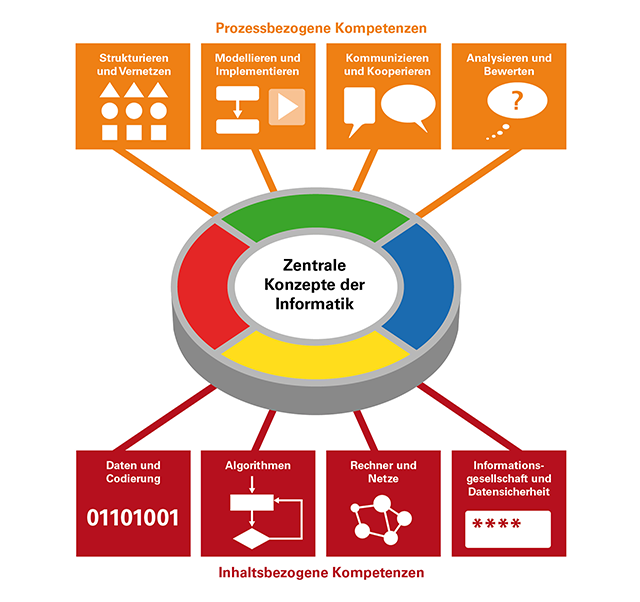
\includegraphics[width=\textwidth,height=\textheight,keepaspectratio]{images/BildungsplanInformatik.png}
	\caption{Infografik zu den Inhalten des Bildungsplans 2016 von Baden-Würtemberg für das Fach Informatik}
	\label{Bildungsplan Infromatik Infografik}
\end{figure}

Im folgenden wird auf die verschieden Kompentenzen eingegangen deren Inhalte, sowie deren Art und Weise wie diese beigebracht werden, erläutert. Leider leifert der Bildungsplan für das Fach informatik keine Beispiele für Unterrichtsmaterialien, weshlab hier nur auf die beschriebenen Inhalte eingegangen wird.

\subsubsection{Strukturieren und Vernetzen}
Mit der Kompetenz Strukturieren und Vernetzen sollen die Schüler lernen wie Daten effizient und strukturiet gespeichert werden können um sie so apäter wieder schnell abrufen zu können. Hierbei lernen die Schüler z.B. wie Daten in einem Graphen, einem Baum oder einer Liste gespeichert werden können. Andererseits beinhaltet diese Kompetenz aber auch Problemlösungen aus dem Alltag zu strukturieren, in Teillösungen aufzuspalten, diese zu Lösen und somit das Gesamtproblem zu lösen.\cite{StruktVer} Im folgenden Schaubild werden die erwarteten Kompetenzen noch einmal aufgelistet:


\begin{figure}[H]
	\centering
	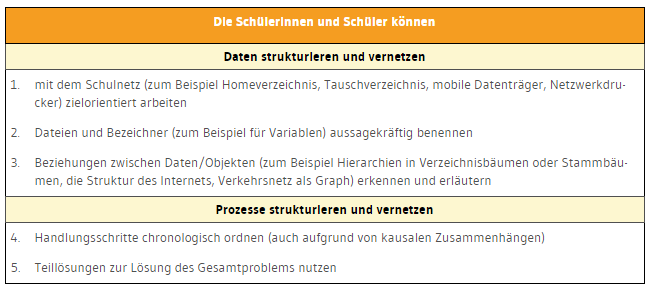
\includegraphics[width=\textwidth,height=\textheight,keepaspectratio]{images/struc.png}
	\caption{Infografik zu den Kompetenzen der Schüler im Fach Informatik im Bereich Strukturieren und Vernetzen}
	\label{Strukturieren und Vernetzen Infografik}
\end{figure}

\subsubsection{Modellieren und Implementieren}

todo umschreiben:
Die Schülerinnen und Schüler können Problemstellungen sowohl der realen Welt als auch aus konstruierten Problemstellungen aufbereiten und daraus informatische Modelle erstellen, diese in einer geeigneten Umgebung implementieren, ihre korrekte Funktionsfähigkeit testen und so funktionsfähige informatische Systeme kreieren.
Sie entwickeln Programme zur Problemlösung. Ausgehend von spielerisch-probierenden Ansätzen gehen sie dabei zunehmend planvoll und strukturiert vor. Sie können Strategien zum Problemlösen auswählen, ihre Auswahl begründen und daraus unter Verwendung von geeigneten Zwischenschritten und/oder Ideenskizzen einen Plan zur Lösung entwickeln. Systematisches Testen, Fehlersuche und Verifizieren eines Ergebnisses sind dabei zunehmend feste Bestandteile des Implementierungsprozesses. Sie untersuchen, inwieweit die Umsetzung den Erfordernissen der Aufgabenstellung/Realsituation entspricht \cite{Model}.

\begin{figure}[H]
	\centering
	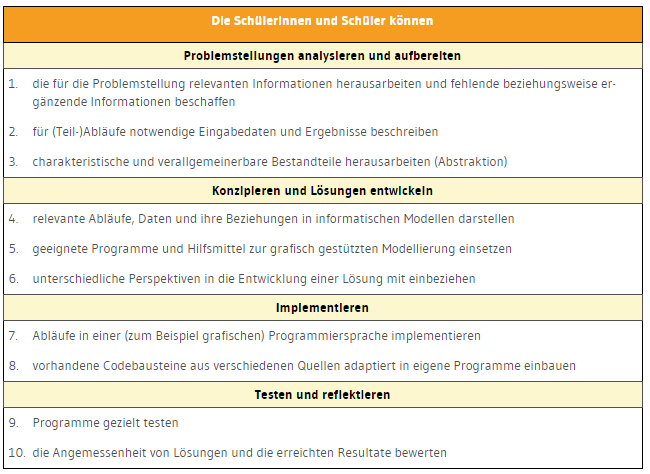
\includegraphics[width=\textwidth,height=\textheight,keepaspectratio]{images/model.png}
	\caption{Infografik zu den Kompetenzen der Schüler im Fach Informatik im Bereich Modellieren und Implementieren}
	\label{Modellieren und Implementieren Infografik}
\end{figure}

\subsubsection{Kommunizieren und Kooperieren}
todo: umschreiben: 
Die Schülerinnen und Schüler erwerben die Fähigkeiten, um informatische Sachverhalte zu diskutieren, zunehmend unter Verwendung von Fachsprache. Sie dokumentieren ihre Ideen, Beobachtungen, Lösungswege und (Teil‑)Ergebnisse und verwenden geeignete Medien und (fachspezifische) Notationsweisen zur Visualisierung. Die Schülerinnen und Schüler nutzen vorhandene Medien und Infrastruktur zur Kommunikation und Kooperation. Sie präsentieren technische Sachverhalte, Arbeitsprozesse und Ergebnisse in geeigneter Form und verwenden dabei eine wertschätzende und geschlechtersensible Sprache.
Sie setzen sich kritisch mit Fragen zum Spannungsfeld zwischen Informatik und Gesellschaft auseinander und beachten in ihrer Arbeitsweise erste rechtliche Aspekte. Dabei zeigen sie einen respektvollen Umgang und Offenheit gegenüber anderen Lösungswegen, Meinungen und Ansichten und diskutieren Aspekte von Toleranz und Akzeptanz von Vielfalt im Kontext informatischer Fragestellungen\cite{Model}.

\begin{figure}[H]
	\centering
	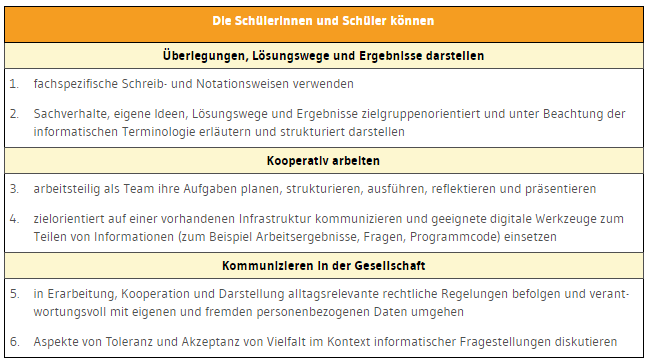
\includegraphics[width=\textwidth,height=\textheight,keepaspectratio]{images/team.png}
	\caption{Infografik zu den Kompetenzen der Schüler im Fach Informatik im Bereich Kommunizieren und Kooperieren}
	\label{Kommunizieren und Kooperieren Infografik}
\end{figure}

\subsubsection{Analysieren und Bewerten}
todo: umschreiben
Die Schülerinnen und Schüler untersuchen eigene und gegebene Programme und informatische Systeme. Die Analyse von Code führt dabei ausgehend von der Identifikation der verwendeten Kontrollstrukturen über ein schrittweises Nachvollziehen des Programmablaufs zum Begreifen der Funktionalität des Programms.
Ihr Wissen über die innere Struktur von Informatiksystemen befähigt sie, Risiken und Chancen einzuschätzen und gegebenenfalls geeignete Sicherheitsmaßnahmen zu ergreifen. Dabei berücksichtigen sie sowohl technische und sicherheitsrelevante als auch gesellschaftliche und ethische Aspekte\cite{Analy}.

\begin{figure}[H]
	\centering
	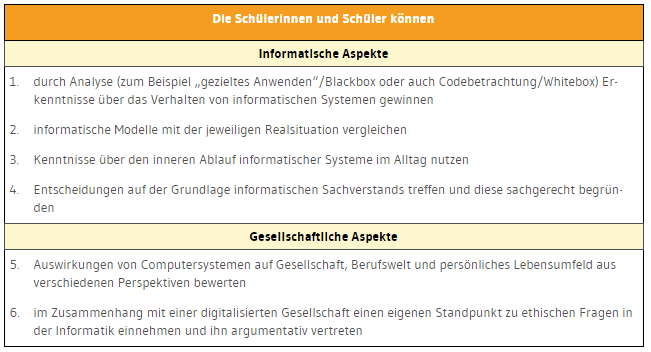
\includegraphics[width=\textwidth,height=\textheight,keepaspectratio]{images/Analysieren.png}
	\caption{Infografik zu den Kompetenzen der Schüler im Fach Informatik im Bereich Analysieren und Bewerten}
	\label{Analysieren und Bewerten Infografik}
\end{figure}

\subsubsection{Daten und Codierung}
todo umschreiben
Die Schülerinnen und Schüler können ausgehend von alltäglichen Codierungen aus ihrem Lebensumfeld (zum Beispiel KFZ-Kennzeichen, Erzeugercode Hühnerei, Barcodes) Elemente der zugrundeliegenden Codierungsvorschriften herausarbeiten. Sie können vorgegebene Codierungen (zum Beispiel Morsecode) anwenden. Sie lernen erste einfache Codierungen durch 0-1-Folgen (zum Beispiel Binärsystem, ASCII-Code) kennen und erfahren dabei an Beispielen, dass Informationen von Maschinen nur dann gespeichert, automatisch verarbeitet oder übertragen werden können, wenn sie in Form von digitalen Daten vorliegen. Allgegenwärtige Größenangaben von Datenmengen (zum Beispiel „8 GB“) erlangen so eine Bedeutung. Die Schülerinnen und Schüler bekommen eine erste Vorstellung davon, dass alle Dateien in Bitfolgen codierte Daten sind\cite{Daten}.

\subsubsection{Algorithemn}
todo: umschreiben
Die Schülerinnen und Schüler lernen ausgehend von Arbeitsabläufen aus ihrer Erfahrungswelt Algorithmen als formalisierte Handlungsanweisungen zur Lösung von Problemen kennen. Sie können Algorithmen mithilfe elementarer Anweisungen und Kontrollstrukturen beschreiben, lernen Variablen als änderbaren Wertespeicher kennen und entwerfen zu gegebenen Problemstellungen erste eigene Algorithmen. Hierbei erfahren sie, dass ein Algorithmus auch für variierende Problemstellungen (zum Beispiel unterschiedliche Anfangswerte, Benutzerinteraktion) geeignet sein muss. Grafische Veranschaulichungen (Struktogramme/Flussdiagramme) erleichtern das Verständnis des Aufbaus von Algorithmen.
Die Schülerinnen und Schüler implementieren Algorithmen in einer geeigneten (zum Beispiel visuellen) Programmierumgebung und können gegebene Algorithmen schrittweise nachvollziehen (zum Beispiel auch zur Fehlersuche). So bekommen sie eine erste Idee von der Funktionsweise eines Computers als „Algorithmen ausführende Maschine“. Dabei lernen sie an Beispielen den Gesamtprozess von der Problemanalyse über das Aufstellen von Algorithmen bis hin zur Implementierung und deren Verifizierung (Testen) kennen.
Ausgehend vom Bewusstsein über im Alltag vorkommende Algorithmen entwickeln die Schülerinnen und Schüler eine Vorstellung von der zunehmenden Bedeutung von Algorithmen in unserer heutigen Welt\cite{Algo}.

\subsubsection{Rechner und Netze}
todo umschreiben

Die Schülerinnen und Schüler beschreiben ausgehend von ihrer Erlebniswelt alltägliche (digitale) Kommunikationsarten und lernen so erste, der digitalen Kommunikation zugrunde liegende Ideen kennen. Grundlegende Strukturen von Netzen ermöglichen einen Einblick in die Hintergründe alltäglich ablaufender Kommunikationsvorgänge im Internet. Sie lernen Endgeräte (auch ihre eigenen) in ihrer Funktion als Teil des Internets kennen. Die Kenntnis über verschiedene Arten von Datenspeicherung und ‑transport ermöglicht so ein tiefergehendes Verständnis von Aspekten der informationellen Selbstbestimmung\cite{Rechner}.

\subsubsection{Informationsgesellschaft und Datensicherheit}
todo umschreiben
Basierend auf dem neu erworbenen Verständnis über Datenspeicherung, ‑verarbeitung und ‑transport sowie der grundlegenden Struktur des Internets, gelangen die Schülerinnen und Schüler zu einem technisch untermauerten Bewusstsein für die Notwendigkeit, Daten gegen unbefugte Nutzung zu schützen. Sie erfahren an konkreten Beispielen, dass in der Informationsgesellschaft neue Anforderungen an Verfügbarkeit, Vertraulichkeit und Integrität von Daten entstehen und jeder Einzelne die Verantwortung für seine Daten übernehmen muss.
Die Schülerinnen und Schüler lernen sowohl einfachste Verschlüsselungsverfahren als auch das Brechen derselben kennen und erhalten so einen ersten Einblick in das Teilgebiet der Kryptologie.
Sie werden dafür sensibilisiert, dass es alltagsrelevante, rechtliche Regelungen gibt.
Vor dem Hintergrund permanent anfallender, personenbezogener Daten werden verschiedene Aspekte der informationellen Selbstbestimmung, insbesondere Datenvermeidung und ‑sparsamkeit beleuchtet, Maßnahmen diskutiert und deren Wirksamkeit in Grundzügen eingeschätzt. Die Schülerinnen und Schüler diskutieren dabei konstruktiv-kritisch auch normative, ethische und soziale Aspekte\cite{InfoGes}.

\subsection{Fazit}
Nach der Erläuterung des aktuellen Bildungsplans sind einige aus der Einleitung genannten Punkte doch breits schon umgesetzt worden. Aberes ist natürlich auch nicht davon ausgehen, dass ein Fach auch genau so unterrichtet wird, wie es im Bildungsplan vorgeschrieben wird. Theorie und Praxis unterscheiden sich in der Realität öfters und es gibt noch viele andere Faktoren die sich auf den Lerninhalt eines Schüler auswriken, wie z.B. Die Kompetenz des Lehrers oder der Wille zu Lernen bei den Schülern. Ein weiterere recht auffälliger Punkt, der bei der AUfkam war, dass der vorherige Bildungsplan zum Bildungsplan 2016 aus dem Jahr 2004 stammt. Wenn dieses Tempo beibehalten wird, kann man nicht vor dem Jahr 2028 mit einem neuen Bildungsplan rechnen. Im Feld der Informatik kann man es sich aber einfach nicht Leisten 12 Jahre lang nichts zu tun, während sich in der neue Technologien entwicklen und neue Paradigmen entstehen, während die alten langsam an relevanz verlieren und schließlich verschwinden. Deshalb sollte sich ein Bildungsplan in deutlich kleineren Abständen erneuern, wenn der Ziel doch sein soll, die nächste Generation auf die Real Welt loszulassen. Ein großer Punkt aus der Einleitung der nicht vom Bildungsplan abgedeckt wird ist eine Form von Logik-Unterricht und allgemein Fächer oder EInheiten in der Grundschule die mit Informatik oder Logik zu tun haben. Deshalb wäre genau das ein Potential das man noch erarbeiten könnte.

\section{Logik-Unterricht in der Grundschule}
dat können die kleinen scheißer auch!